
\documentclass{article}

% Lenguaje y Fuente
\usepackage[spanish]{babel}
\usepackage[utf8x]{inputenc}
\usepackage[T1]{fontenc}
\usepackage[top=1in, bottom=1.25in, left=1.1 in, right=1.1 in]{geometry}
\usepackage{graphicx}
\usepackage{ragged2e}
\usepackage[usenames]{color}
\usepackage{multicol}

% Portada

\title{\textbf{Reporte de la Actividad 2}\\ Introducción a Python y Jupyter Lab}
\author{Luis Fernando Duarte Gonzalí \\ Universidad de Sonora \\ Física Computacional}
\date{Febrero del 2019}
\begin{document}
\maketitle

% Contenido del Reporte

\section{Introducción}

\noindent En el siguiente trabajo el objetivo es introducirnos a la biblioteca de \textit{Pandas} en Python, específicamente en el entorno de \textsc{Jupyter Lab}. Además de probar nuestra comprensión de lectura de textos en inglés, el manejo de Jupyter Lab y de archivos de datos.

Se analizará un archivo descargado del Servicio Meteorológico Nacional, en concreto la ciudad de León en Guanajuato, México usando el archivo medias y extremas diarias responderemos a preguntas planteadas para un correcto análisis de datos.

\section{Climatología}

La climatología es la rama de las Ciencias de la Tierra que se ocupa del estudio del clima y sus variaciones a lo largo del tiempo cronológico. Ha sido un asunto del que se había ocupado la geografía desde sus comienzos: Claudio Ptolomeo, en su libro "Geographia", dedica un tercio de éste a la variación zonal de los climas en la superficie terrestre.

Aunque utiliza los mismos parámetros que la meteorología (ciencia que estudia el tiempo atmosférico), su objetivo es distinto, ya que no pretende hacer previsiones inmediatas, sino estudiar las características climáticas a largo plazo.

De las condiciones atmosféricas dependen muchas actividades humanas, desde la agricultura hasta un simple paseo por el campo. Por eso se ha hecho un esfuerzo ingente por predecir el tiempo tanto a corto como a medio plazo.

\subsection{Subgerencia de Pronóstico a Mediano y Largo Plazo}

La Subgerencia de Pronóstico a Mediano y Largo Plazo (SPMLP) es la subdivisión de la Gerencia de Meteorología y Climatología de la Coordinación General del Servicio Meteorológico Nacional, encargada de proveer información climática útil para el país. En esta Subgerencia se mantienen los siguientes proyectos actualmente:

\begin{itemize}
    \item Pronóstico Estacional: Desarrolla la perspectiva de temperatura y precipitación de las variaciones del tiempo a mediano plazo a tres meses. Analizando las condiciones existentes y las proyecciones de acuerdo a pronósticos de tipo estadísticos y dinámicos consultados y desarrollados por la misma área.
    
    \item Diagnóstico Climático: Desarrolla las actualizaciones del monitoreo del fenómeno del ENOS, también se mantiene realizando los diagnósticos de las condiciones climáticas existentes en el mediano plazo.
    
    \item Monitor de Sequía: Desarrolla productos quincenales y mensuales que proporcionan un resumen general de las condiciones de sequía en el país y en América del Norte. Por medio de múltiples indicadores de sequía, incluyendo varios índices, perspectivas, informes de campo y otros que son revisados por especialistas para elaborar los productos.
    
    \item Climatología, Calidad y Optimización de datos: En conjunto se encargan de mantener y actualizar la base de datos climática Nacional realizando la revisión de registros climáticos y pruebas de control de calidad.
\end{itemize}

\section{Análisis de Datos}

Para comenzar, necesitamos abrir \textsc{Jupyter Lab} desde Anaconda Prompt, abriendo la carpeta creada previamente con el nombre de \textit{Actividad3}.
Una vez abierto, en python, primero se importaron las bibliotecas Pandas, Numerical Python y Matplot para generar las gráficas.

\begin{center}
    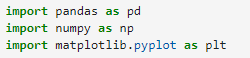
\includegraphics[scale = 1]{Librerias.png}
\end{center}

\noindent Se leyó el archivo de texto, definiéndole una variable, también se saltaron los renglones innecesarios que fueron 4 para después estructurar los datos de mejor manera con \textit{DataFrame}.

\begin{center}
    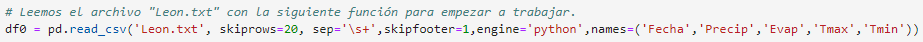
\includegraphics[scale = .65]{read.png}
    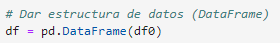
\includegraphics[scale = .8]{DataFrame.png}
\end{center}

Para que python pudiera leer los archivos nulos, fue necesario reemplazar la palabra \textit{Nulo} por NaN. Además de cambiar los tipos de datos para poder trabajar con ellos.
\begin{center}
    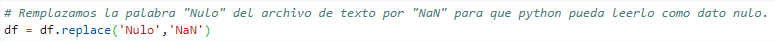
\includegraphics[scale = .74]{NaN.png}
    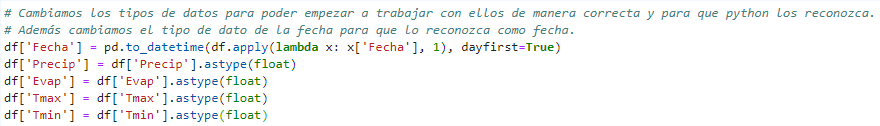
\includegraphics[scale = 0.65]{Float.png}
\end{center}

\section{Resultados}
Para comenzar a mostrar los resultados, primero tenemos que plantearnos las preguntas correctas. Buscamos determinar cuáles son los meses más lluviosos, también nos preguntamos cuáles son los meses más cálidos y fríos, podemos preguntarnos cuáles han sido los años más húmedos y los más secos, otra cosa que podemos visualizar son los inviernos más fríos y los veranos más cálidos. De alguna manera podemos ver la temperatura mensual promedio en los últimos veinte años así como el comportamiento de las lluvias en esos mismos años.

\subsection{Precipitación}
Para determinar cuáles son los meses más lluviosos se puede generar una gráfica donde se muestre la precipitación como función del tiempo. Para poder visualizar los meses más lluviosos se usó el siguiente código agrupando, desde la columna \textsc{Fecha}, los meses.

\subsubsection{Suma de las Precipitaciones por Mes}
\begin{center}
    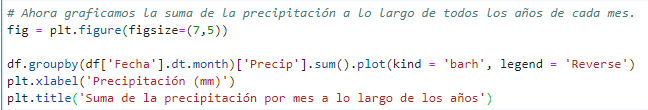
\includegraphics[scale = 0.80]{SumPrecip.png}
\end{center}
Que nos generó la siguiente gráfica:
\begin{center}
    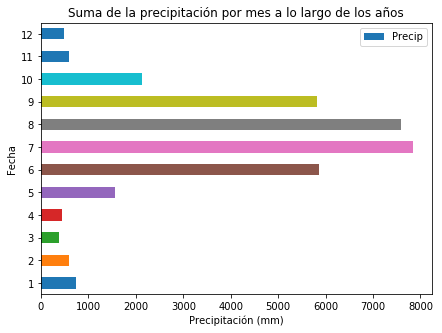
\includegraphics[scale = 0.55]{GSumPrecip.png}
\end{center}
Donde se puede observar que los meses con más lluvias son desde junio hasta septiembre.

\subsubsection{Precipitación Media Anual}
En la siguiente gráfica podemos ver la precipitación media anual en la ciudad de León, con este gráfico podemos responder a la pregunta de cuáles han sido los años más húmedos al igual que los más secos.
\begin{center}
    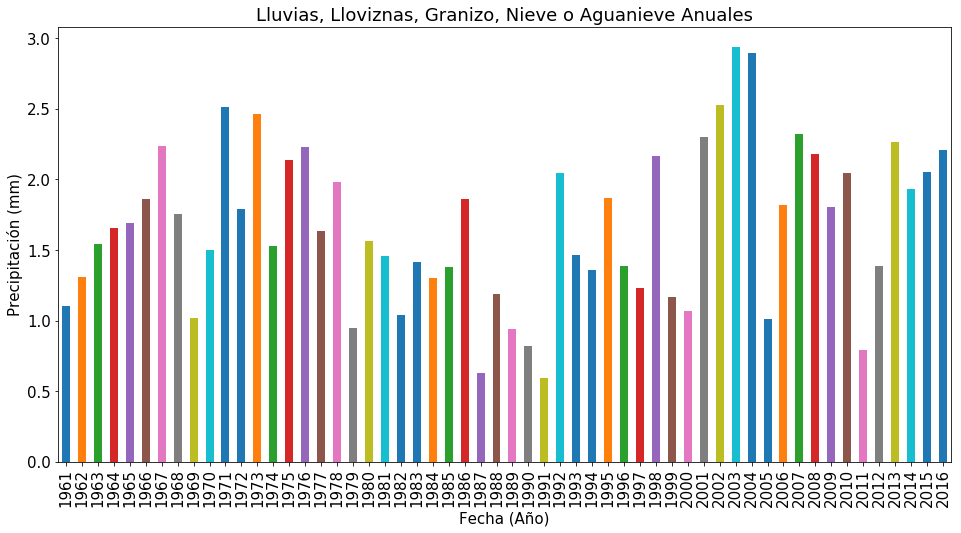
\includegraphics[scale = 0.47]{GLluvia.png}
\end{center}
En la gráfica anterior se pueden observar muchas fluctuaciones, pero también podemos notar unos picos muy altos que representan los años más lluviosos o húmedos que son del 2001 al 2004 donde el 2003 ha sido el año más húmedo. En el sentido contrario podemos observar que los años más secos fueron del 1987 al 1991 y el más reciente 2011.

\subsubsection{Precipitación Media Anual en los últimos 20 años}

Centrándonos en los últimos 20 años de datos que van desde 1997 hasta el 2016 de precipitación media podemos ver que ha cambiado bastante, todos los años son muy diferentes en esta región de la república, no siguen cierto patrón o algo por el estilo.

\begin{center}
    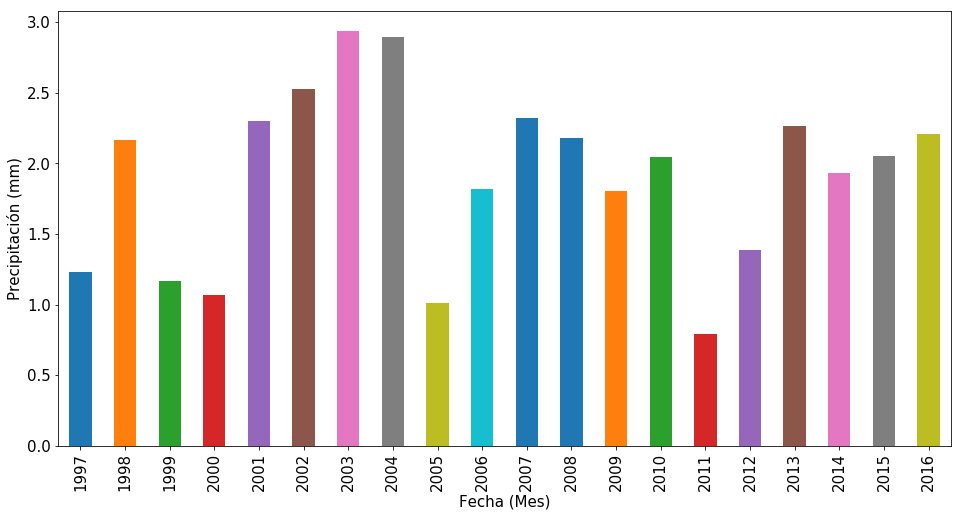
\includegraphics[scale = 0.46]{Last20Precip.png}
\end{center}


\subsection{Temperatura}
Para responder a la pregunta de cuáles fueron los meses más cálidos y los más fríos podemos hacerlo visualizando una gráfica que nos muestre los valores promedio de la temperatura máxima y mínima a través de los años.

\subsubsection{Promedio de las Temperaturas Mínimas y Máximas}
Para generar las gráficas se utilizó un código bastante parecido, que se muestran a continuación:
\begin{center}
    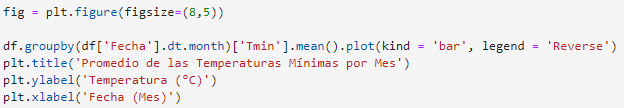
\includegraphics[scale = 0.6]{Tmin.png}
    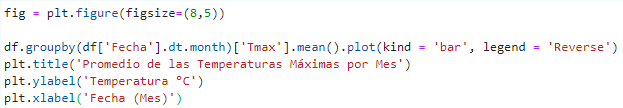
\includegraphics[scale = 0.6]{Tmax.png}
\end{center}

\clearpage

Las gráficas generadas del promedio de las temperaturas mínimas y máximas por mes por el código son las siguientes:
\begin{figure}[h]
\centering
  \begin{minipage}{0.4\textwidth}
    \centering
    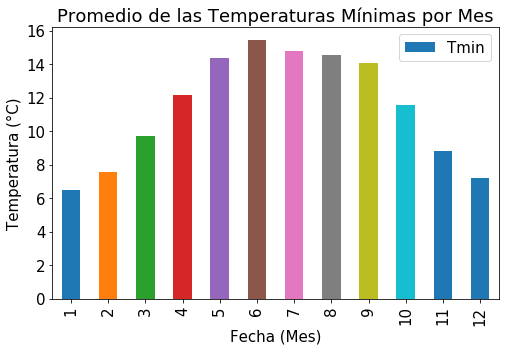
\includegraphics[width=1\textwidth]{GTmin.png}
  \end{minipage}
  \hspace{5mm}
  \begin{minipage}{0.4\textwidth}
    \centering
    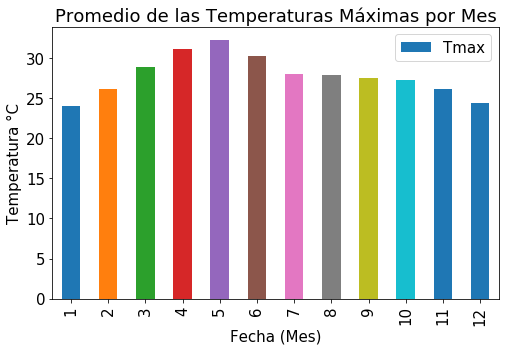
\includegraphics[width=1\textwidth]{GTmax.png}
  \end{minipage}
\end{figure}

Donde se puede observar de manera muy clara que la temperatura máxima en León, Guanajuato no cambia mucho a lo largo de todo el año, aunque gracias a la gráfica de la temperatura mínima podemos observar los meses más cálidos del año, que por lo general se encuentran en verano (21 de junio al 23 de Septiembre aproximadamente) que se encuentra cerca de los 15°C como mínima y poco arriba de los 25°C como máxima. De igual manera podemos ver que los meses más fríos son los que abarca el invierno, es decir, entre diciembre y marzo donde las temperaturas mínimas rondaron entre los 6°C y 9°C, y las altas entre 23°C y poco menos de 29°C.

\subsubsection{Temperatura Mensual Promedio en los últimos 20 años}
\begin{figure}[h]
\centering
  \begin{minipage}{0.4\textwidth}
    \centering
    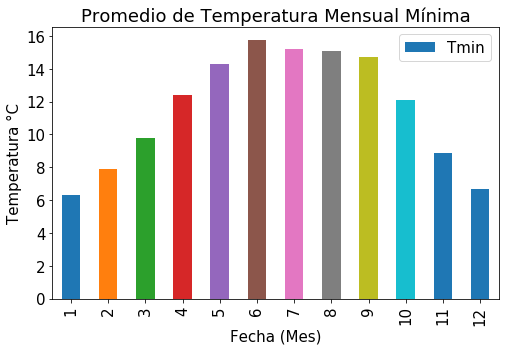
\includegraphics[width=1\textwidth]{GTmin20.png}
  \end{minipage}
  \hspace{5mm}
  \begin{minipage}{0.4\textwidth}
    \centering
    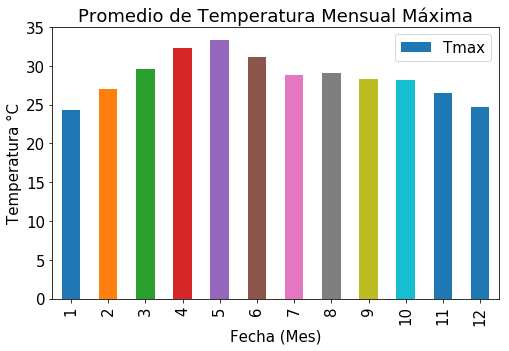
\includegraphics[width=1\textwidth]{GTmax20.png}
  \end{minipage}
\end{figure}
Se puede observar que la forma de la gráfica es muy parecida a la del total de los datos.

\section{Conclusión}

Se ha logrado llegar al objetivo perseguido durante la actividad de manera algo lenta, pero segura. Al momento de hacer el análisis, para mí fue mejor trabajar con las gráficas porque es mucho más intuitivo ver barras que representen cierta cantidad de algún parámetro que se desea estudiar. Se me ha complicado un poco encontrar cada función para agregar y responder de manera correcta a las preguntas planteadas para hacer un buen análisis de los datos.

\clearpage

\section{Bibliografía}
\begin{itemize}

    \item Servicio Meteorológico Nacional. (2019). Consultado: 9 de Febrero del 2019, de Conagua. Sitio web: http://smn1.conagua.gob.mx/emas/
    
    \item Python Tutorial (2019). Consultado: 10 de Febrero del 2019, de tutorialspoint. Sitio web:
    
    https://www.tutorialspoint.com/python/index.htm
    
    \item Análisis y visualización de datos con Pandas \& MatPlotLib. (2018). Consultado: 12 de Febrero del 2019, de Code Like a Girl. Sitio web:
    
    https://code.likeagirl.io/an\%C3\%A1lisis-y-visualizaci\%C3\%B3n-de-datos-con-pandas-matplotlib-85ee4d7b4cad
    
    \item Biblioteca Pandas. (2019). Consultado: 10 de Febrero del 2019, de Pandas Pydata. Sitio web: https://pandas.pydata.org/pandas-docs/stable/index.html
    
    \item Agrupación de datos por fecha en pandas. (2018). Consultado: 12 de Febrero del 2019, de Analytics Lane. Sitio web:
    
    https://www.analyticslane.com/2018/07/06/agrupacion-de-datos-por-fecha-en-pandas/
    
    \item 10 minutes to Pandas. (2019). Consultado 11 de Febrero del 2019, de Pandas Pydata. Sitio web: http://pandas.pydata.org/pandas-docs/stable/getting\_started/10min.html\#min
    
    \item Agrupar Filas por Mes y Año. (2016). Consultado: 11 de Febrero del 2019, de stackoverrun. Sitio web:
    
    https://stackoverrun.com/es/q/10689859
\end{itemize}








\end{document}
